\documentclass[12pt, notitlepage, final]{article}

\newcommand{\name}{Vince Coghlan and Zach Vogel}

%\usepackage[dvips]{graphics,color}
\usepackage{amsfonts}
\usepackage{amssymb}
\usepackage{amsmath}
\usepackage{latexsym}
\usepackage{enumerate}
\usepackage{amsthm}
\usepackage{nccmath}
\usepackage{setspace}
\usepackage[pdftex]{graphicx}
\usepackage{epstopdf}
\usepackage[siunitx]{circuitikz}
\usepackage{tikz}
\usepackage{float}
\usepackage{cancel}
\usepackage{setspace}
\usepackage{overpic}
\usepackage{mathtools}
\usepackage{listings}
\usepackage{color}
\usepackage{qtree}
\usepackage{pgfplots}
\usepackage{pdflscape}
\usepackage{rotating}
%\usepackage{gensymb}

\usetikzlibrary{calc}
\usetikzlibrary{matrix}
\usetikzlibrary{positioning}

%\numberwithin{equation}{section}
\newcommand{\dbr}[1]{d_{\mbox{#1BR}}}
\newtheorem{lemma}{Lemma}
\newtheorem*{corollary}{Corollary}
\newtheorem{theorem}{Theorem}
\newtheorem{proposition}{Proposition}
\theoremstyle{definition}
\newtheorem{define}{Definition}

\newdimen\digitwidth{}
\settowidth\digitwidth{0}
\def~{\hspace{\digitwidth}}

\setlength{\parskip}{1pc}
\setlength{\parindent}{0pt}
\setlength{\topmargin}{-3pc}
\setlength{\textheight}{9.0in}
\setlength{\oddsidemargin}{0pc}
\setlength{\evensidemargin}{0pc}
\setlength{\textwidth}{6.5in}

\DeclareMathOperator*{\argmin}{arg\,min}

%absolute value code
\DeclarePairedDelimiter\abs{\lvert}{\rvert}%
\DeclarePairedDelimiter\norm{\lVert}{\rVert}
\makeatletter
\let\oldabs\abs{}
\def\abs{\@ifstar{\oldabs}{\oldabs*}}
%
\let\oldnorm\norm{}
\def\norm{\@ifstar{\oldnorm}{\oldnorm*}}
\makeatother

\def\dbar{{\mathchar'26\mkern-12mu d}}
%\def \P[x]{\Frac{\partial}{\partial x}}
%\def \D[x]{\Frac{d}{dx}}
\newcommand{\PD}[2]{\frac{\partial#1}{\partial#2}}
\newcommand{\PF}[1]{\frac{\partial}{\partial#1}}
\newcommand{\DD}[2]{\frac{d#1}{d#2}}
\newcommand{\DF}[1]{\frac{d}{d#1}}
\newcommand{\fix}[2]{\left(#1\right)_#2}
\newcommand{\ket}[1]{|#1\rangle}
\newcommand{\bra}[1]{\langle#1|}
\newcommand{\braket}[2]{\langle{} #1 | #2 \rangle}
\newcommand{\bopk}[3]{\langle{} #1 | #2 | #3 \rangle}
\newcommand{\Choose}[2]{\displaystyle{} {#1 \choose{} #2}}
\newcommand{\proj}[1]{\ket{#1}\bra{#1}}
\def\del{\vec{\nabla}}
\newcommand{\avg}[1]{\langle#1\rangle}
\newcommand{\piecewise}[4]{\left\{\beginProtected{array}{rl}#1&:#2\\#3&:#4\endProtected{array}\right.}
\newcommand{\systeme}[2]{\left\{\beginProtected{array}{rl}#1\\#2\endProtected{array}\right.}
\def\Godel{G$\ddot{\mbox{o}}$del}

\title{Cache Simulator}
\date{\today}
\author{\name}

\begin{document}

\maketitle


\section{Introduction}

Cache configurations are not a one size fits all job.  Some cache's are better than others for specific
applications.  For example, a multiway cache will benifit a system that has limited space, as hit rates
will increase.  A direct-mapped cache will be better for a larger cache, since our hit times will be very
fast.  Our simulations are an attempt to discover some of these facts.  We created a simulator that will
preform instruction, read, and write operations on any associativity or size cache.  This cache system
included a hierarchy of a level 1 instruction cache, a level 1 data cache, and a unified level two cache.
The caches are all write-allocate, write-back, meaning writes will immidiately write to the cache, and any
data in the cache that has been written must be accounted for and lazily written back down to level two and
eventually main memory.  All caches maintain their own Least Recently Used (LRU) policy in order to preform
the best that they can given information at any point in execution.  We measured many metrics, such as hit
time, miss time, cost, CPI, ideal times, and kickouts.  Although many things are idealized, this simulator
is very similar to what you would see in a modern computing machine.

\section{Design}
There were several design considerations of note that must be addressed.  The first concern of ours, was one
of memory.  The stack was stored as an array of structures in heap memory.  This was mainly for speed reasons.
An array is generally faster than a linked list when we dont know where in the list we are going.  The second
consideration was how to design the requests.  We found it to be simplist to split the simulator, much like a
computer does, into the CPU portion, and the cache portion.  The CPU decides how many references it needs, and
decides what to do when it gets a hit, miss, or dirty kickout.  The cache portion, on the other hand, was a
simple machine.  It took the address and the cache it was looking in and that is essentially it.  It returned
a hit, miss, or the tag of a dirty kickout that it received.  The CPU simulater then decides what to do with
this information.  The last important consideration was the LRU system.  We knew that the fastest solution
would be to provide each block with a number that would represent it's place in the LRU.  This would be a
constant time solution.  This, however, led to some difficulties in implementation when we had variable sized
caches.  We instead went with a linked list structure.  This made it easy to program, and we knew that for
every cache other than the fully associative, this time would be relatively minimal.

The use of the code is quite simple.  The inluded makefile will build the program on our versions of Mac OSX
10.9 and Arch Linux.  just typing make is sufficient, while make clean will remove the compiled files.  The
libraries used are quite simple.  libc and the POSIX standard library are all that is required.  Once built
the program will be called cachesim.  At that point it can be run with an option describing some features.
cachesim -v will run in "verbose" mode, where each cache reference and clock cycle will be spelled out step
by step.  Besides helping in debugging, it is quite relaxing to watch all the text fly by.  cachesim -h will
print out the usage: "usage: cat $<$traces$>$ $|$ ./cachesim [-hv] $<$config\_file$>$".  Note that the traces
must be sent in through stdin, any other form of stdin will work as well, not just cat.  The config file takes
the form of a series of lines, each with a parameter, followed by a space, then a value.  For example, a line
could be "l1dassoc 4".  That would set the level 1 data cache to a 4-way set associative cache.  A full list
can be seen in the code, or in the example config files provided.

\section{Simulation}
The simulations were run on multiple cores of a PC running Debian Linux virtualized in a windows enviornment.
In total they were run in a little under 20 hours.  The simulations included a number of traces that tested
a variaty of typical operations a computer would run.  Not suprisingly the simulations of the fully
associative caches took almost twice as long as the direct mapped ones.  The LRU's linked list had to be
traversed and reorganized on almost every reference.  This meant slow references, as well as a much less
efficient real-life cache.  We simluated each of the 5 traces on 10 different caches.  Additionally, the
omnetpp simulation was run on systems with multiple memory chunk sizes from cache to main memory.  We will
preform cost benifit analysis on this later.

\section{Results}
The best way to present this data, in our minds, is to represent it as a ratio of the real time over the
ideal time.  Since many of the traces vary in ideal execution time, but are mostly proportional to the
stack parameters, the best option to initally analyse the data is to average out the values from each
group of traces and present the ratio over ideal time.  This can be seen below.

\begin{center}
\begin{tikzpicture}
\begin{axis}[
    ybar,
    enlargelimits=0.15,
    title=Execution Time Proportional to Ideal Execution Time,
    ylabel=Ratio Compared to Ideal,
    legend style={at={(0.5,-0.2)},
      anchor=north,legend columns=-1},
    symbolic x coords={default, l1-2way, all-2way, l2-4way, all-4way, l2-big, l1i-small, l1d-small, l1-small, all-FA},
    xtick=data,
    nodes near coords,
	    nodes near coords align={vertical},
    x tick label style={rotate=45,anchor=east},
    width=16cm,
    height=12cm
]
\addplot
coordinates {(default, 17.26) (l1-2way, 15.14) (all-2way, 15.16) (l2-4way, 14.17)
(all-4way, 13.38) (l2-big, 12.62) (l1i-small, 18.14) (l1d-small, 20.52)
(l1-small, 21.53) (all-FA, 12.13)};
\end{axis}
\end{tikzpicture}
\end{center}

The two fastest caches are all-FA and l2-big and, unsuprisingly, the slowest caches are the ones with smaller
l1 cache sizes.  We know that a fully associative cache will gaurantee the highest hit rate.  If we had a very
high miss penalty this would be our best bet, since we would always hit.  The larger L2 cache will also
guarantee a low l2 miss rate which means, less accesses to main memory, the slowest part of the process.

There are reasons why we dont use these caches for our everyday computing.  The fully associative simulation
does not take into account the amount of time it takes to move down the LRU list and update it on every
reference.  It is also extremely expensive, as we will show later on.  The large L2 cache is sufficient to
allow more hits of older data.  This is great, but comes at the cost of a larger cache.

Cost considerations are very important when considering which cache to choose.  If we manufacture processors,
what matters to us is the bottom line, profit.  The ratio of perfomance over cost can be seen below.

\begin{center}
\begin{tikzpicture}
\begin{axis}[
    ybar,
    enlargelimits=0.15,
    title=Execution Time Proportional to Ideal Execution Time,
    ylabel=Ratio Compared to Ideal,
    legend style={at={(0.5,-0.2)},
      anchor=north,legend columns=-1},
    symbolic x coords={default, l1-2way, all-2way, l2-4way, all-4way, l2-big, l1i-small, l1d-small, l1-small, all-FA},
    xtick=data,
    nodes near coords,
	    nodes near coords align={vertical},
    x tick label style={rotate=45,anchor=east},
    width=16cm,
    height=12cm
]
\addplot
coordinates {(default, 0.000110357) (l1-2way, 0.0000714056) (all-2way, 0.00006765442) (l2-4way, 0.00006885037)
(all-4way, 0.00005244801) (l2-big, 0.00008127108) (l1i-small, 0.000129710097) (l1d-small, 0.0001146657)
(l1-small, 0.0001429132) (all-FA, 0.00001974616)};
\end{axis}
\end{tikzpicture}
\end{center}



\end{document}
